\chapter{模型改进部分}

上一章介绍了生成个对抗网络和扩散模型的基本思想,以及实际中分别常用的DCGAN、DDPM模型。然而,在掌静脉数据增强实验中DCGAN模型和DDPM模型都存在一定的问题:
DCGAN出现了GAN技术常见的模式崩溃(生成器仅覆盖真实分布的部分模式)、训练震荡(生成器和判别器无法收敛到稳定均衡)问题。
DDPM在实验中虽然可以生成高质量图片,但对高信噪比掌静脉图像的去噪学习效果不佳(部分)。
为此,本文结合相关文献内容\cite{salimans2016improved}\cite{10323353}\cite{nichol2021improved},分别对DCGAN和DDPM进行了掌静脉图像数据增强的技术改进。

\section{DCGAN改进:标签平滑化、特征匹配技术}

\subsection{信息不对称博弈}
生成对抗网络(GAN)\cite{goodfellow2014generative}是一类基于博弈论的潜变量生成模型。
GAN的目标是训练生成器网络$G(z;\theta^{(G)})$,以至于可以利用向量噪声$z$生成符合真实数据分布$p_{data}(x)$的样本。
生成器$G$的训练信号由判别器网络$D(x)$提供,该网络经过训练以区分来自生成器分布$p_{model}(x)$的样本和真实数据。
然后,生成器网络G反过来被训练以欺骗判别器接受其输出是真实的。GAN的应用表明,它们可以产生出色的样品\cite{denton2015deep}。

从博弈论的观点来看,训练GAN实现损失函数的最小化,就是找到生成器和判别器两者博弈的纳什均衡
\footnote{在博弈论中,纳什均衡(Nash equilibrium)是指在包含两个或以上参与者的非合作博弈中,假设每个参与者都知道其他参与者的均衡策略的情況下,沒有参与者可以通过改变自身策略使自身受益时的一个概念解}。
在达到纳什均衡时,生成器与判别器都无法通过参数更新实现获益(损失降低)。

对生成器与判别器组成的博弈关系,如果其所有策略可以由损失矩阵$\mathbf{M}\in\mathbb{R}^{m\times n}$完全给出。
其中,$m$是生成器可能的博弈策略数量,$n$是判别器可能的博弈策略数量。当生成器选择策略$i$并且判别器选择策略$j$时,$M_{ij}$是生成器的损失(或等价于判别器的收益)
那么根据冯诺依曼极小极大定理,GAN基于交替优化的策略可以完全达到\textbf{博弈值}$\mathbf{p^TMq}$

\begin{theorem}[Vonneumunn极小极大定理]
    \label{the:vonn}
    对于任意由博弈损失矩阵$\mathbf{M}\in\mathbb{R}^{m\times n}$定义的有限的两个体零和博弈,有下式成立:
    \[
    \underset{p}{\min}\underset{q}{\max}\mathbf{p^TMq}=\underset{q}{\max}\underset{p}{\min}\mathbf{p^TMq}
    \]
\end{theorem}

然而,GAN中生成器与判别器通常由深度神经网络组成,两者的博弈是建立在具有\textbf{连续高维参数}的\textbf{非凸}策略空间(参数空间)上的,这意味着存在多个局部博弈均衡点而非唯一的全局鞍点。
此外生成器与判别器之间的博弈属于信息不对称的竞争,这种不对称体现在下面几个方面:

1)生成器的信息劣势:生成器掌握自身参数和生成数据的分布规律(例如如何从潜在空间映射到数据空间),但无法直接观测真实数据的完整分布。它需要通过与判别器的交互,间接学习如何调整生成策略。

2)判别器的局部信息:判别器通过真实数据和生成器输出的混合样本进行训练,但它无法直接获取生成器的参数或生成过程的内部机制。随着训练的进行,判别器会逐渐捕捉生成数据的统计特征,但这种信息获取是滞后的。

3)优化不同步:生成器和判别器的信息优势是交替变化的。当判别器改进时,生成器被迫调整策略以生成更逼真的数据,从而再次打破判别器的信息优势。这种动态博弈导致信息不对称不断被打破和重建,而非静态以损失矩阵的形式存在。

GAN通常使用梯度下降算法(如SGD,RMSprop,Adam等)进行网络参数更新,这些技术旨在找到损失函数的低值,而不是找到策略对抗的纳什均衡。
当用于寻找纳什均衡时,这些算法可能无法收敛\cite{goodfellow2014generative}。
因此,为了解决生成器与判别器之间的不对称博弈问题,本文参考相关文献\cite{salimans2016improved},采用标签平滑化技术和特征匹配技术两种策略,增加对抗信息,在一定程度上改善对抗训练的信息缺失。

\subsection{标签平滑化}
标签平滑技术\cite{szegedy2016rethinking}\cite{10323353}将负标签0和真标签1目标替换为平滑值(如0.9或0.1),以增强神经网络对样本标签判断结果的学习,优化反向传播方法对参数的更新效果。
定义用$\alpha$替换正判别的标签,$\beta$替代负判别的标签,这样判别器
\begin{equation}
    \label{eq:smooth}
    D(x)=\frac{\alpha p_{data}(x)+\beta p_{model}(x)}{p_{data}(x)+p_{model}(x)}
\end{equation}
在\autoref{eq:smooth}分子中的$p_{model}$是不应该存在的,因为这意味着在$p_{data}(x)$较小而$p_{model}(x)$较大的区域错误样本会让$D(x)\approx\beta$,使得错误样本的分布也在靠近$p_{data}(x)$,而这是不符合目的。
因此通常会设定$\beta=0$,而将正判别的标签平滑为$\alpha$,这种技术通常也被称为\textbf{单侧标签平滑化}。

\subsection{特征匹配}
特征匹配的思想起于使用最大均值差异来训练网络\cite{dziugaite2015training}\cite{li2015generative}。该方法通过为生成器指定新目标来防止在当前判别器上的过度训练,改善了GAN的训练不稳定性。
生成器的新目标并不是直接最大化判别器的输出,而是要求生成器生成与真实数据的统计数据匹配的数据,使用判别器来指定值得匹配的统计数据。

具体来说,通常会选择训练生成器以匹配判别器中间层上特征的预期值。
生成器需要拟合正样本在判别器中间特征层的分布,以实现特征匹配的目的。这种做法充分利用了判别器网络中间特征层,克服了生成器的信息劣势。

本文基于特征匹配的思想,在掌静脉数据增强任务中,令$f(x)$表示判别器某中间层上的激活层结果,生成器的新目标定义为
\begin{equation}
    \underset{\theta}{argmin}\Big[V(G^{(\theta)},D)+\big|\big|\mathbb{E}_{x\sim p_{data}(x)}f(x)-\mathbb{E}_{z\sim p_{z}(x)}f(G(z;\theta))\big|\big|_1\Big]
\end{equation}
作为二分类任务的判别器目标不变,仍然是生成样本、真实样本分别与负、正标签的交叉熵损失之和,按梯度下降法进行参数更新训练。

\section{DDPM改进:余弦加噪过程替换线性加噪过程}
虽然扩散模型DDPM的生成图像质量高,但是使用DDPM技术的掌静脉数据增强相关研究还比较少见。原因包括:DDPM采样步骤长,训练速度缓慢,对计算机算力需求高。
本文实验中也由于算力不足,只选取了掌静脉图像中心的128x128尺寸的静脉图像做预处理,压缩为32x32分辨率的掌静脉局部图像实验DDPM生成效果。实验图片参见\autoref{fig:palmvein}

根据相关文献\cite{nichol2021improved},扩散模型的线性加噪过程技术适用于高分辨率照片,对于64x64和32x32的低分辨率照片则表现不佳。
原因是在低分辨率的图片中,有效图像信息被压缩,信噪比增大。在32x32的低分辨率掌静脉图像前向过程里,表现为为掌静脉结构被噪声快速破坏的情况,参见\autoref{fig:linearnoise}。
这种情况在部分静脉图案不明显,纹理结构不清晰的图片上更加严重。可见不管是低分辨率图片生成,还是高信噪比的掌静脉图像数据增强,线性加噪方式都不是最佳选择。

\begin{figure}[!htbp]
    \centering
    \includegraphics[width=10cm]{image/chap04/linear_noise.jpg}
    \caption{掌静脉图像线性加噪过程}
    \label{fig:linearnoise}
\end{figure}

\subsection{余弦加噪方式}
线性加噪过程也存在算力浪费,反向扩散过程冗长的情况。相关文献\cite{nichol2021improved}中在反向扩散过程跳过超百分之二十的步骤后,模型的生成效果并没有变差(FID
\footnote{FID:Frechet Inception Distance。是一种使用广泛的评估生成图像质量的度量标准
FID是通过计算两个分布之间的Fréchet距离来衡量生成模型和真实数据分布之间的差异。Fréchet距离是一种度量两个分布之间距离的方法,它考虑到了两个分布的均值和协方差矩阵,可以更好地描述两个分布之间的差异。
在计算FID时,首先从真实数据分布和生成模型中分别抽取一组样本,然后使用预训练的Inception网络从这些样本中提取特征向量。接下来,计算两个分布的均值和协方差矩阵,并计算它们之间的Fréchet距离,得到FID值。FID值越小,表示生成模型生成的图像越接近于真实数据分布。
}无明显增加)。
为了改善这些问题,一种新的加噪方式——余弦加噪方式被提出。余弦加噪方式如其名,使用余弦函数来平缓$\bar{\alpha}_t$趋向于0的速度,参见\autoref{fig:contrast2}。

\begin{equation}
    \label{eq:cos2noise}
    \bar{\alpha}_t=\frac{f(t)}{f(0)},f(t)=\cos\Big(\frac{t/T+s}{1+s}\times\frac{\pi}{2}\Big)^2
\end{equation}
我们注意到$\beta_t=1-\dfrac{\bar{\alpha}_t}{\bar{\alpha}_{t-1}}$,因此在实践中,为了避免$\beta_t=1$的情况发生,通常会进行截断0.999。
\autoref{eq:cos2noise}中的超参数$s$能够避免$\beta_t$在$t=0$时过小。过小的早期噪声会影响神经网络对噪声预测,损失显著增大。

\begin{figure}[!htbp]
    \centering
    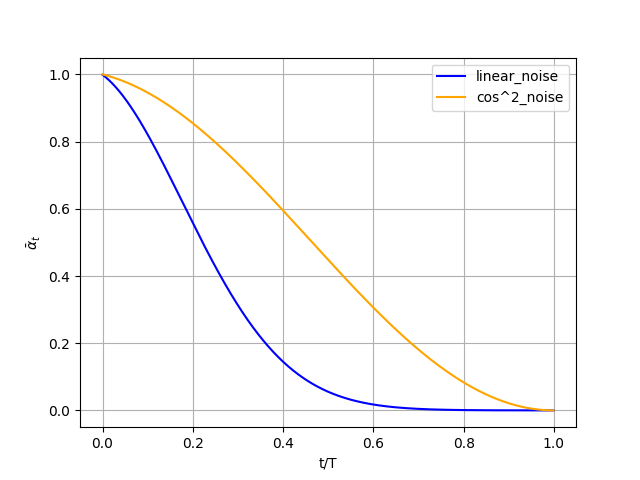
\includegraphics[width=10cm]{image/chap03/contrast2.png}
    \caption{线性加噪与余弦加噪对比}
    \label{fig:contrast2}
\end{figure}

然而在掌静脉图像生成实验中发现,余弦加噪确实可以减缓图片纹理被破坏的速度,但神经网络预测噪声的困难变大,体现为预测误差增大近一倍(MSE:1.23$\rightarrow$2.37),在100epochs后仍无法准确反向采样出有效图片。

本文对加噪过程的改进基于余弦加噪函数进行微调,综合了线性加噪与余弦加噪的优势。目的使加噪声过程平缓,同时让每一步噪声差异更明显,提高神经网络对噪声的预测准确率。
三种加噪方式(分别是线性加噪,余弦加噪,改进的余弦加噪)在采样过程中参数$\bar{\alpha}_t$的变化如\autoref{fig:contrast3}所示。
\begin{equation}
    \label{eq:cos4noise}
    \bar{\alpha}_t=\frac{f(t)}{f(0)},f(t)=\cos\Big(\frac{t/T+s}{1+s}\times\frac{\pi}{2}\Big)^4
\end{equation}
对比\autoref{eq:cos2noise}和\autoref{eq:cos4noise}可以发现,区别只在于调整了cos函数的次数(从平方调整为四次方),同时在测试中发现超参数选择$s=0.1$效果较良好。

\begin{figure}[!htbp]
    \centering
    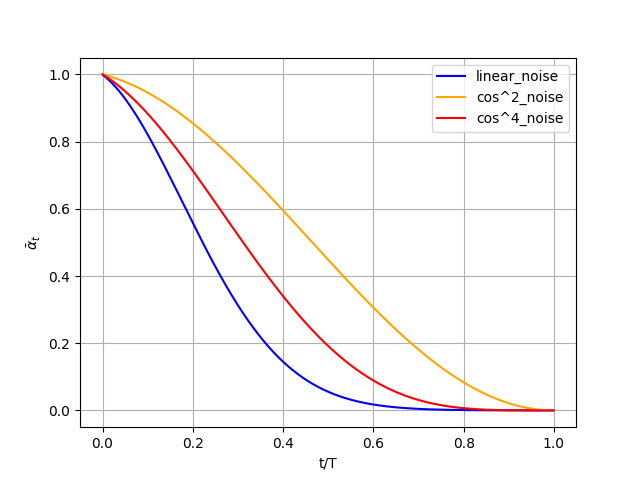
\includegraphics[width=10cm]{image/chap03/contrast3.png}
    \caption{线性加噪、余弦加噪与改进的余弦加噪对比}
    \label{fig:contrast3}
\end{figure}
在掌静脉局部图像上测试三种不同的加噪方式,结果如\autoref{fig:multi-image-noisify}所示。
改进的余弦加噪方式相比线性加噪方式延缓了图像纹理被破坏的速度,与余弦加噪方式相比又有更明显的早期噪声,更利于神经网络训练。

\begin{figure}[h!]
    \centering
    % 第一组图文
    \parbox{10cm}{\centering (a) 线性加噪} \\  % 文字说明
    \includegraphics[scale = 0.15]{image/chap03/linear_noise.jpg} \\
    % 第二组图文
    \parbox{10cm}{\centering (b) 改进的余弦加噪} \\  % 文字说明
    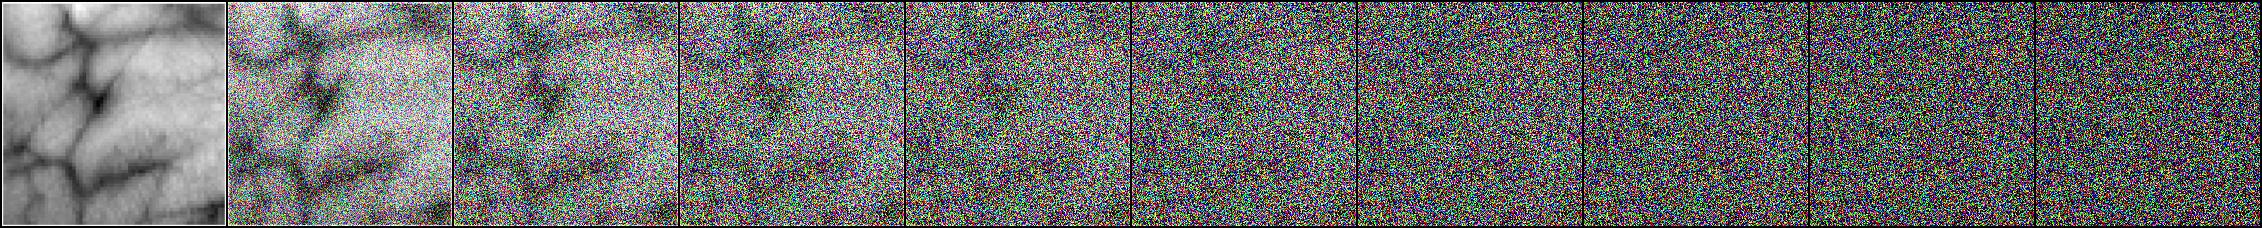
\includegraphics[scale = 0.15]{image/chap03/cos^4_noise.jpg} \\
    % 第三组图文
    \parbox{10cm}{\centering (c) 余弦加噪} \\  % 文字说明
    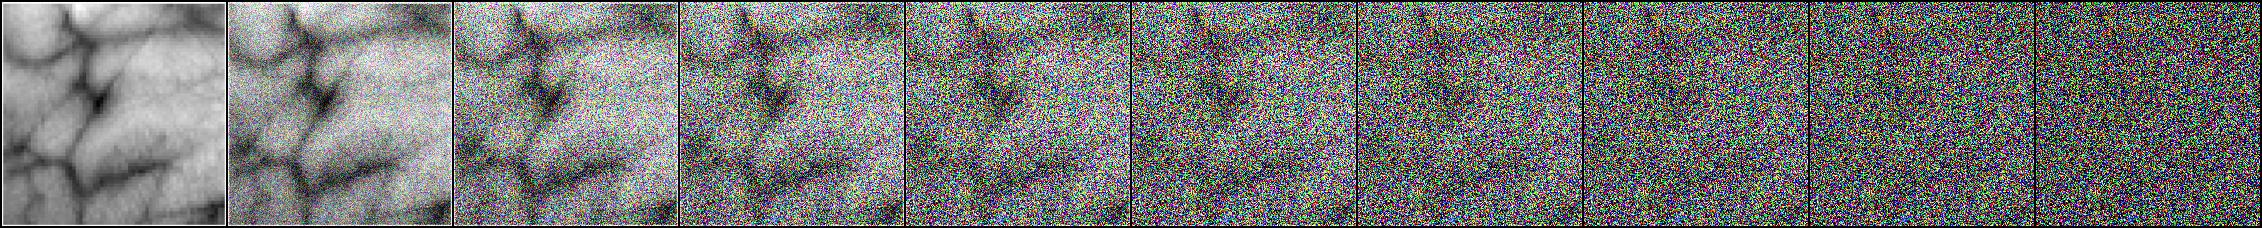
\includegraphics[scale = 0.15]{image/chap03/cos^2_noise.jpg}
    
    \caption{不同加噪图像方式对比}
    \label{fig:multi-image-noisify}
\end{figure}
